\begin{figure}[ht]
\centering
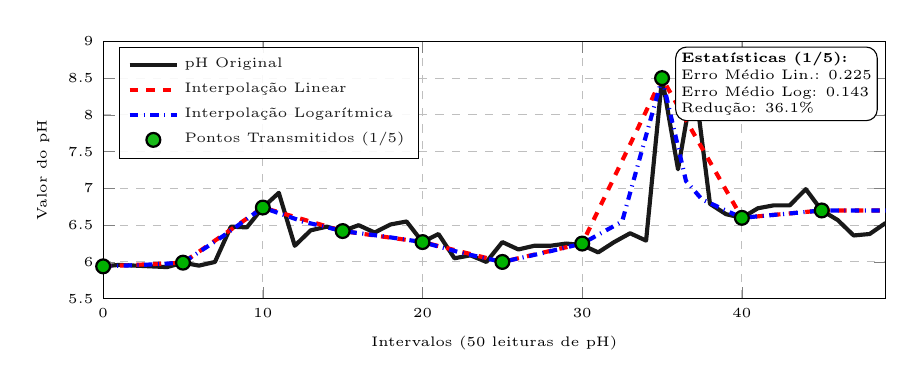
\begin{tikzpicture}
\begin{axis}[
    % --- DIMENSÕES E ESTILOS GERAIS (Mantidos) ---
    width=0.95\textwidth,
    height=0.40\textwidth,
    grid=major,
    tick label style={font=\tiny},
    label style={font=\tiny},
    grid style={dashed, gray!50},
    % --- CONFIGURAÇÃO DA LEGENDA (Alterada) ---
    legend cell align=left,
    legend style={
        at={(0.02,0.98)}, % Posição interna: canto superior esquerdo com pequena margem
        anchor=north west, % Ancoragem pelo canto superior esquerdo da caixa
        legend columns=1,  % Uma coluna (lista vertical)
        font=\tiny,        % Fonte pequena
        draw=black,        % Borda preta na caixa
        fill=white,        % Preenchimento branco
        fill opacity=0.9   % Ligeira transparência para ver a grade atrás, se necessário
    },
    % --- CONFIGURAÇÕES ESPECÍFICAS DOS DADOS DE PH ---
    xlabel={Intervalos (50 leituras de pH)},
    ylabel={Valor do pH},
    xmin=0, xmax=49,
    ymin=5.5, ymax=9.0,
    xtick={0, 10, 20, 30, 40},
    ytick={5.5, 6.0, 6.5, 7.0, 7.5, 8.0, 8.5, 9.0},
]

% --- PLOTS DE DADOS (Conteúdo mantido) ---

% 1. pH Original
\addplot[color=black!90, line width=1.5pt, line join=round] coordinates {
    (0, 5.94) (1, 5.96) (2, 5.95) (4, 5.93) (5, 5.99) 
    (6, 5.95) (7, 6.00) (8, 6.48) (9, 6.47) (10, 6.74) 
    (11, 6.94) (12, 6.22) (13, 6.43) (14, 6.48) (15, 6.42) 
    (16, 6.50) (17, 6.40) (18, 6.51) (19, 6.55) (20, 6.27) 
    (21, 6.38) (22, 6.05) (23, 6.09) (24, 6.00) (25, 6.27) 
    (26, 6.17) (27, 6.22) (28, 6.22) (29, 6.25) (30, 6.23) 
    (31, 6.13) (32, 6.27) (33, 6.39) (34, 6.29) (35, 8.50) 
    (36, 7.26) (37, 8.51) (38, 6.79) (39, 6.65) (40, 6.60) 
    (41, 6.73) (42, 6.77) (43, 6.77) (44, 6.99) (45, 6.70) 
    (46, 6.57) (47, 6.36) (48, 6.38) (49, 6.53)
};
\addlegendentry{pH Original}

% 2. Interpolação Linear
\addplot[color=red, dashed, line width=1.5pt] coordinates {
    (0, 5.94) (5, 5.99) (10, 6.74) (15, 6.42) (20, 6.27) 
    (25, 6.00) (30, 6.25) (35, 8.50) (40, 6.60) (45, 6.70) (49, 6.70)
};
\addlegendentry{Interpolação Linear}

% 3. Interpolação Logarítmica
\addplot[color=blue, dashdotted, line width=1.5pt] coordinates {
    (0, 5.94) (2.5, 5.96) (5, 5.99) (7.5, 6.35) (10, 6.74) 
    (12.5, 6.55) (15, 6.42) (17.5, 6.35) (20, 6.27) (22.5, 6.12) 
    (25, 6.00) (27.5, 6.12) (30, 6.25) (32.5, 6.55) (35, 8.50) 
    (36.5, 7.1) (37.5, 6.85) (40, 6.60) (42.5, 6.65) (45, 6.70) (49, 6.70)
};
\addlegendentry{Interpolação Logarítmica}

% 4. Pontos Transmitidos
\addplot[only marks, mark=*, mark options={fill=green!70!black, draw=black, line width=0.8pt, mark size=2.5pt}] coordinates {
    (0, 5.94) (5, 5.99) (10, 6.74) (15, 6.42) (20, 6.27) 
    (25, 6.00) (30, 6.25) (35, 8.50) (40, 6.60) (45, 6.70)
};
\addlegendentry{Pontos Transmitidos (1/5)}

% --- Caixa de Estatísticas (Mantida no canto superior direito) ---
\node[draw=black, fill=white, rounded corners, anchor=north east, font=\tiny, align=left, inner sep=2pt] 
    at (rel axis cs: 0.99, 0.98) {
    \textbf{Estatísticas (1/5):}\\
    Erro Médio Lin.: 0.225\\
    Erro Médio Log: 0.143\\
    Redução: 36.1\%
};

\end{axis}
\end{tikzpicture}
\caption{Interpolação Linear vs Interpolação Logarítmica}
\label{fig:interpolacao-linear-vs-log}
\end{figure}
